\documentclass{article}

\PassOptionsToPackage{numbers,compress,sort}{natbib}
\usepackage[preprint]{neurips_2023}

\usepackage[utf8]{inputenc}
\usepackage[T1]{fontenc}
\usepackage{hyperref}
\usepackage{url}
\usepackage{booktabs}
\usepackage{amsmath,amssymb,amsfonts}
\usepackage{nicefrac}
\usepackage{microtype}
\usepackage{xcolor}
\usepackage{graphicx}
\usepackage{multirow}
\usepackage{enumitem}
\usepackage{tikz}
\usetikzlibrary{arrows.meta,positioning,fit,calc}
\usepackage{pgfplots}
\pgfplotsset{compat=1.18}
\usepackage{subcaption}
\usepackage{fontawesome5}
\usepackage[capitalise,noabbrev]{cleveref}

% Course header instead of the NeurIPS notice.
\makeatletter
\renewcommand{\@noticestring}{EECE 576L (Fall 2026), University of British Columbia. Course project proposal.}
\makeatother

\newcommand{\R}{\mathbb{R}}
\newcommand{\SO}{\mathrm{SO}(3)}
\newcommand{\SE}{\mathrm{SE}(3)}
\newcommand{\so}{\mathfrak{so}(3)}
\newcommand{\Log}{\operatorname{Log}}
\newcommand{\Exp}{\operatorname{Exp}}
\newcommand{\method}{\textsc{I2P-Flow}}
\newcommand{\ph}{\textcolor{gray}{--}}   % placeholder cell
\definecolor{phgray}{gray}{0.55}

\setlist{itemsep=1pt,topsep=2pt,parsep=0pt}
\setlength{\textfloatsep}{8pt plus 2pt minus 2pt}
\setlength{\intextsep}{6pt plus 2pt minus 2pt}
\setlength{\abovecaptionskip}{3pt}

\title{\method: Riemannian Flow Matching for\\Camera Localization in LiDAR Maps}

\author{%
  Sibo Ma\\
  Department of Electrical and Computer Engineering\\
  University of British Columbia, Vancouver, Canada\\
  \texttt{masibo@student.ubc.ca}
}

\begin{document}
\maketitle

% =====================================================================
\begin{abstract}
Image-to-point-cloud (I2P) registration, locating a camera in a LiDAR point cloud, lets cheap cameras localize in accurate LiDAR maps.
Recent progress comes mostly from better cross-modal matching, and every method still outputs a \emph{single} pose, typically by solving Perspective-n-Point with RANSAC (PnP-RANSAC). A single pose cannot express ambiguity, such as the position along a straight highway or between look-alike places.
We propose \method{}, a pose head that replaces PnP-RANSAC with conditional \emph{Riemannian flow matching} on $\SO\times\R^3$ that samples the camera pose given the image and point cloud. Each refinement step conditions the velocity on image features sampled where the LiDAR points project under the current pose.
On KITTI and nuScenes, we evaluate whether it matches PnP-RANSAC accuracy while giving calibrated uncertainty, measured by negative log-likelihood (NLL), coverage and failure detection.
A matched Gaussian head, a highway hold-out and a synthetic twin-place benchmark then test whether its gains come from representing multiple modes.
\end{abstract}

% =====================================================================
\section{Introduction}
\label{sec:intro}

Autonomous vehicles and robots must know their full 6-DoF pose, often in urban canyons, tunnels or indoor spaces where GNSS is unreliable. Since dense LiDAR maps are increasingly available and cameras cost far less than LiDARs, \emph{camera localization in a LiDAR map} lets a fleet build the map once and localize with commodity sensors, by matching a 2D image against 3D geometry with no shared appearance. The core task is \emph{image-to-point-cloud (I2P) registration}: given an image $I$ with known intrinsics $K$ and a LiDAR point cloud $P$, estimate the rigid transform $T=(R,t)\in\SE$ that maps $P$ into the camera frame, i.e.\ the camera pose in the point-cloud frame.

Deep I2P registration has advanced quickly. On the standard KITTI protocol~\cite{geiger2012kitti}, accuracy at 5$^\circ$/2\,m rose from 83\% (VP2P~\cite{zhou2023vp2p}) to 97.5\% (ICLI2P~\cite{li2025icli2p}). Most of this progress comes from better cross-modal matching, while the pose is still solved with standard PnP-RANSAC; the few methods that change this step, such as ICLI2P's direct regression, still output \emph{one} pose. Map-based localizers such as CMRNet~\cite{cattaneo2019cmrnet,cattaneo2025cmrnext} likewise refine a single estimate.

A single pose is the wrong output when several poses fit the evidence, e.g.\ along a featureless highway or at look-alike intersections. RANSAC then picks one arbitrarily, regression averages the modes, and neither gives uncertainty a downstream filter can use. With KITTI accuracy near its ceiling, knowing \emph{when} the pose is wrong, and what the alternatives are, remains an open problem.

\textbf{Planned contributions.} (1) A conditional Riemannian flow-matching head~\cite{lipman2023flow,chen2024riemannian} on $\SO\times\R^3$ that replaces PnP-RANSAC on a frozen I2P backbone, with \emph{pose-dependent projective conditioning}: at each step, the LiDAR points are projected into the image using the current pose, and the velocity is predicted from the point features together with the image features at those pixels. (2) A controlled test of \emph{why} it helps: a Gaussian head with identical features and conditioning reveals whether gains come from representing multiple modes.

% =====================================================================
\section{Related work}
\label{sec:related}

\textbf{I2P registration.}
Most methods predict 2D--3D correspondences and solve for the pose with PnP-RANSAC~\cite{ren2022corri2p,kang2024cofii2p}.
VP2P-Match~\cite{zhou2023vp2p} trains through a probabilistic PnP layer and ICLI2P~\cite{li2025icli2p} regresses the pose directly, while CMRNet~\cite{cattaneo2019cmrnet} refines an initial guess by comparing the image with the projected map.
Diffusion has been used only as a feature prior~\cite{mu2025diff2i2p} or to refine camera--LiDAR extrinsics~\cite{ou2025diffcalib}; Diff$^2$I2P also reports that supervising the transformation directly was unstable, which motivates supervising the predicted velocity rather than the final pose.
All of these return one pose, and the main uncertainty estimate, evidential regression on CMRNet~\cite{vaghi2022uncertainty}, is unimodal.
We instead return samples and evaluate whether they are calibrated and capture several modes.

\textbf{Pose distributions.}
Parametric heads (Gaussian, EPro-PnP~\cite{chen2022epropnp}) have one peak; Implicit-PDF~\cite{murphy2021ipdf} is multimodal but grid-based, which scales poorly to 6-DoF.
Flow matching~\cite{lipman2023flow,liu2023rectified} extends to manifolds~\cite{chen2024riemannian}.
Flow matching and diffusion over poses have been used for object pose~\cite{jin2025se3poseflow}, relative and multi-view camera pose~\cite{kuczkowski2026posefm,tran2026quacamfm,wang2023posediffusion}, point-cloud registration~\cite{jiang2023se3diffreg} and LiDAR localization~\cite{wang2025bevdiffloc,krummenacher2025diffpr}.
We reuse this machinery. What is new is the cross-modal setting, re-projection conditioning, and the calibration and ambiguity analysis.

% =====================================================================
\section{Method}
\label{sec:method}

\begin{figure}[t]
\centering
\begin{tikzpicture}[
  font=\scriptsize, >={Stealth[length=3.5pt]},
  box/.style={draw, rounded corners=2pt, align=center, minimum height=7mm, inner sep=3pt},
  frz/.style={box, fill=blue!7},
  new/.style={box, fill=orange!15},
]
% inputs and frozen encoders
\node[box, minimum width=11mm] (img) {Image $I$};
\node[box, minimum width=11mm, below=5mm of img] (pc) {LiDAR $P$};
\node[frz, minimum width=17mm, right=3mm of img] (ei) {Image enc.\ \textcolor{blue!70!black}{\faSnowflake}};
\node[frz, minimum width=17mm, right=3mm of pc] (ep) {Point enc.\ \textcolor{blue!70!black}{\faSnowflake}};
\draw[->] (img)--(ei); \draw[->] (pc)--(ep);
% flow step
\node[new, right=12mm of $(ei.east)!0.5!(ep.east)$] (proj) {$\pi\big(K(R_\tau p_j+t_\tau)\big)$\\[1pt]$\to$ tokens $z_j$};
\node[new, right=4mm of proj] (g) {$g_\theta(z,\tau)$ \textcolor{red!80!black}{\faFire}\\[1pt]$\to(\hat\omega,\hat v)\in\R^6$};
\node[new, right=4mm of g] (up) {$R_\tau\Exp(\Delta\tau\,\hat\omega)$\\[1pt]$t_\tau+\Delta\tau\,\hat v$};
\coordinate (mx) at ($(ei.east)!0.65!(ei.east -| proj.west)$);
\draw[->] (ei.east) -- node[below,pos=0.5,inner sep=1.5pt]{$F_I$} (mx) |- ([yshift=1.5mm]proj.west);
\draw[->] (ep.east) -- node[above,pos=0.5,inner sep=1.5pt]{$\{f_j\}$} (ep.east -| mx) |- ([yshift=-1.5mm]proj.west);
\draw[->] (proj)--(g); \draw[->] (g)--(up);
\draw[->] (up.south) |- node[pos=0.75,below,inner sep=1pt]{$T_{\tau+\Delta\tau}$} ([yshift=-3mm]proj.south) -- (proj.south);
\coordinate (lb) at ([yshift=-5mm]proj.south);
\node[draw, dashed, rounded corners=3pt, inner sep=2mm, fit=(proj)(g)(up)(lb), label={[anchor=south east,inner sep=1pt,xshift=-1.5mm]north east:$\times K$}] (loop) {};
% prior and output
\node[box, above=3mm of proj] (prior) {$T_0$};
\draw[->] (prior)--(proj);
\node[box, anchor=west] (out) at ([xshift=4mm]loop.east |- up.east) {$\{T^{(n)}\}_{n=1}^{N}$};
\draw[->] (up.east)--(out.west);
\end{tikzpicture}
\caption{\method{} overview. Frozen encoders map $I$ and $P$ to features $F_I$ and $\{f_j\}$. Starting from a random pose $T_0$, each of $K$ steps projects the points under the current pose $T_\tau$ to form tokens $z_j$, from which $g_\theta$ predicts $(\hat\omega,\hat v)\in\R^6$ to update the pose. $N$ random starts give $N$ samples approximating $p(T\mid I,P)$.}
\label{fig:overview}
\end{figure}


\textbf{Setup and flow matching.}
Our goal is to sample from $p(T\mid I,P)$, the distribution of poses $T=(R,t)$ consistent with image $I$ and point cloud $P$ (\cref{fig:overview}).
Flow matching learns a velocity field that moves a random pose (time $\tau=0$) to a plausible one ($\tau=1$); it is trained on paths from random poses to ground-truth poses.
We treat rotation and translation separately, on $\SO\times\R^3$~\cite{yim2023framediff,bose2024foldflow}.
For a training pair with ground-truth pose $(R_1,t_1)$, we sample a random rotation $R_0\sim\mathrm{Unif}(\SO)$, a translation $t_0\sim\mathcal N(0,\sigma_t^2\mathbf{I}_3)$ and a time $\tau\sim\mathcal U[0,1]$.
Using body-frame (right) multiplication, the geodesic interpolant~\cite{chen2024riemannian} is
\begin{equation}
\begin{aligned}
  R_\tau&=R_0\Exp(\tau\omega^\star), &\quad \omega^\star&=\Log(R_0^\top R_1)=\tfrac{1}{1-\tau}\Log(R_\tau^\top R_1),\\
  t_\tau&=(1-\tau)t_0+\tau t_1, &\quad v^\star&=t_1-t_0,
\end{aligned}
\end{equation}
where $\Exp/\Log$ map between $\R^3\cong\so$ and $\SO$~\cite{sola2018micro}.
Both target velocities, angular $\omega^\star$ and translational $v^\star$, are constant along the path.
A network $g_\theta$ predicts the 6-D velocity $(\hat\omega,\hat v)=g_\theta(z,\tau)$ from tokens $z=z(R_\tau,t_\tau;I,P)$ (defined below), and we train it with
\begin{equation}
  \mathcal L_{\mathrm{FM}}=\mathbb E\big[\|\hat\omega-\omega^\star\|^2+\lambda\|\hat v-v^\star\|^2\big].
\end{equation}
Here $\lambda$ balances the rotational (radians) and translational (meters) terms so that neither dominates.

\textbf{Pose-dependent projective conditioning.}
Frozen encoders give an image feature map $F_I$ and per-point features $f_j$.
At each step, every point is projected under the current pose, $u_j=\pi(K(R_\tau p_j+t_\tau))$, and its token $z_j$ combines $f_j$, the image feature $F_I(u_j)$ at that pixel, and its depth and visibility.
A small transformer $g_\theta$ reads the tokens, so each step acts like a render-and-compare update~\cite{cattaneo2019cmrnet}.

\textbf{Sampling.}
We run $N$ random starts through $K$ Euler steps, $R\!\leftarrow\!R\Exp(\Delta\tau\hat\omega)$, $t\!\leftarrow\!t+\Delta\tau\hat v$, and cluster the $N$ samples into modes. The top mode gives the single pose estimate. \Cref{tab:todo} lists the planned tasks.


\begin{table}[t]
\centering\scriptsize
\caption{To-do list with estimated hours.}
\label{tab:todo}
\begin{tabular}{@{}rlr@{}}
\toprule
\# & Task & Hours \\
\midrule
1 & Data setup (KITTI, nuScenes); reproduce the PnP-RANSAC baseline & 12\\
2 & Implement flow matching on $\SO\times\R^3$ and projective conditioning; first KITTI run & 25\\
3 & Evaluation metrics and baselines (Gaussian head, VP2P-Match) & 15\\
4 & Ambiguity experiments (highway hold-out, twin places) and ablations & 15\\
5 & Presentation & 6\\
6 & Final report and code release & 20\\
\midrule
 & \textbf{Total} & \textbf{93} \\
\bottomrule
\end{tabular}
\end{table}

% =====================================================================
\section{Experiments}
\label{sec:exp}

\textbf{Setup.}
On KITTI Odometry~\cite{geiger2012kitti} we use the standard I2P protocol~\cite{ren2022corri2p,kang2024cofii2p}: train on sequences 00--08 and test on 09--10, with a random up-axis rotation and a ground-plane offset of up to 10\,m applied to the point cloud.
On nuScenes~\cite{caesar2020nuscenes} we use the CoFiI2P split.
We report both registration accuracy (Acc: relative rotation error (RRE) $<5^\circ$ and relative translation error (RTE) $<2$\,m) and registration recall (RR: $<10^\circ$, $<5$\,m), plus median RTE and RRE.
Uncertainty metrics are negative log-likelihood (NLL), empirical coverage of highest-posterior-density (HPD) regions, the area under the receiver operating characteristic curve (AUROC) for failure detection, and mode recall.
Baselines are CoFiI2P + PnP-RANSAC using its inlier ratio and a PnP-Jacobian covariance as uncertainty, VP2P-Match~\cite{zhou2023vp2p}, and a Gaussian head that shares our features, tokens and transformer but outputs one pose with a covariance, so it differs only in whether several modes can be represented.

\subsection{Accuracy on KITTI and nuScenes}
\emph{Goal:} show that sampling does not cost accuracy (\cref{tab:main}).
\emph{Expected:} the top mode is within a few points of CoFiI2P+RANSAC in Acc.

\begin{table}[h]
\centering\scriptsize
\caption{Main results. $\dagger$: published numbers with a different backbone.}
\label{tab:main}
\begin{tabular}{@{}lcccccccc@{}}
\toprule
 & \multicolumn{4}{c}{KITTI Odometry (seq.\ 09--10)} & \multicolumn{4}{c}{nuScenes} \\
\cmidrule(lr){2-5}\cmidrule(lr){6-9}
Method & RTE (m)$\downarrow$ & RRE ($^\circ$)$\downarrow$ & Acc (\%)$\uparrow$ & RR (\%)$\uparrow$ & RTE & RRE & Acc & RR \\
\midrule
GraphI2P$^\dagger$ / ICLI2P$^\dagger$ / DPA-I2P$^\dagger$ & \ph & \ph & \ph & \ph & \ph & \ph & \ph & \ph \\
VP2P-Match & \ph & \ph & \ph & \ph & \ph & \ph & \ph & \ph \\
CoFiI2P + PnP-RANSAC (reproduced) & \ph & \ph & \ph & \ph & \ph & \ph & \ph & \ph \\
Gaussian head (same backbone + cond.) & \ph & \ph & \ph & \ph & \ph & \ph & \ph & \ph \\
\method{} (top mode) & \ph & \ph & \ph & \ph & \ph & \ph & \ph & \ph \\
\bottomrule
\end{tabular}
\end{table}

\subsection{Calibration and failure detection}
\emph{Goal:} test whether the predicted spread matches the actual error (\cref{fig:calib}a,b).
\emph{Expected:} \method{} has the lowest NLL and coverage closest to the diagonal.
The RANSAC covariance is likely over-confident on failures, and the Gaussian head over-dispersed on ambiguous frames.

\begin{figure}[h]
\centering
\pgfplotsset{every axis/.style={width=0.355\linewidth,height=0.27\linewidth,tick label style={font=\tiny},label style={font=\scriptsize},title style={font=\scriptsize,yshift=-1ex},legend style={font=\tiny,inner sep=1pt,row sep=-2pt}}}
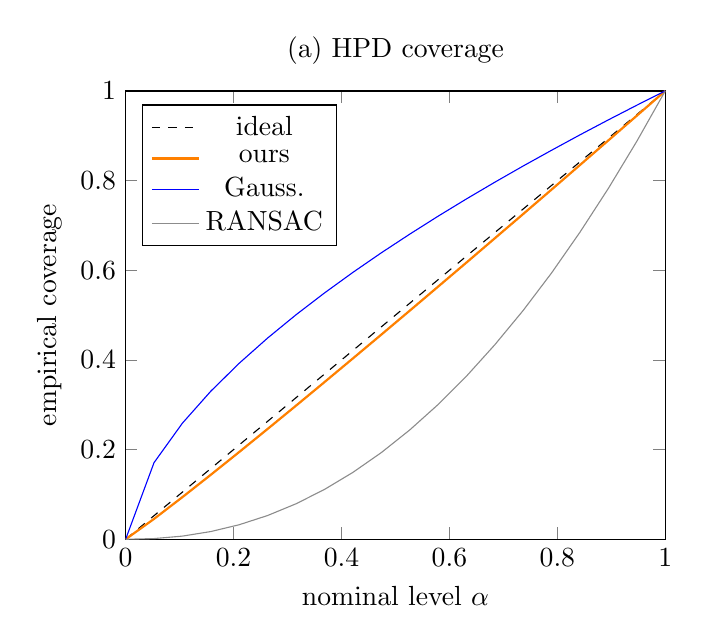
\begin{tikzpicture}
\begin{axis}[title={(a) HPD coverage}, xlabel={nominal level $\alpha$}, ylabel={empirical coverage}, xmin=0,xmax=1,ymin=0,ymax=1, legend pos=north west]
\addplot[black,dashed,domain=0:1] {x}; \addlegendentry{ideal}
\addplot[orange,thick,domain=0:1,samples=20] {x^1.05}; \addlegendentry{ours}
\addplot[blue,domain=0:1,samples=20] {x^0.6}; \addlegendentry{Gauss.}
\addplot[phgray,domain=0:1,samples=20] {x^2.2}; \addlegendentry{RANSAC}
\end{axis}
\end{tikzpicture}\hfill
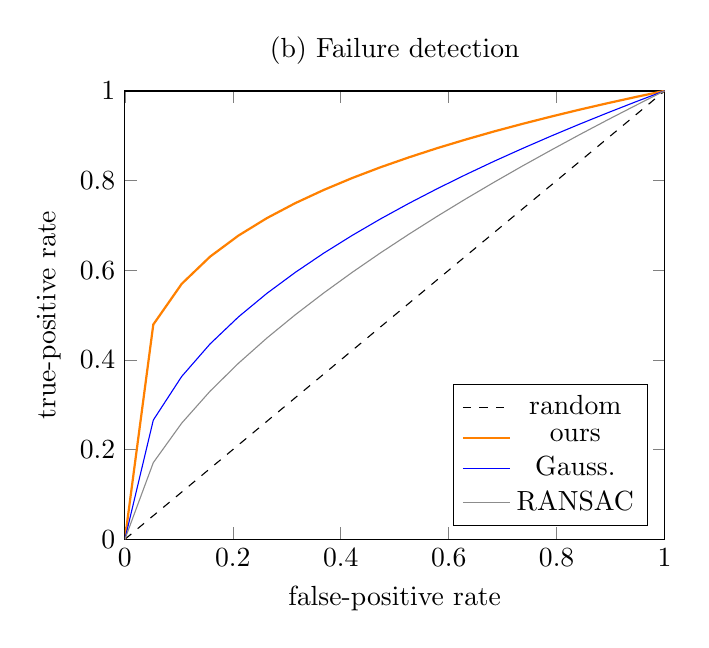
\begin{tikzpicture}
\begin{axis}[title={(b) Failure detection}, xlabel={false-positive rate}, ylabel={true-positive rate}, xmin=0,xmax=1,ymin=0,ymax=1, legend pos=south east]
\addplot[black,dashed,domain=0:1] {x}; \addlegendentry{random}
\addplot[orange,thick,domain=0:1,samples=20] {x^0.25}; \addlegendentry{ours}
\addplot[blue,domain=0:1,samples=20] {x^0.45}; \addlegendentry{Gauss.}
\addplot[phgray,domain=0:1,samples=20] {x^0.6}; \addlegendentry{RANSAC}
\end{axis}
\end{tikzpicture}\hfill
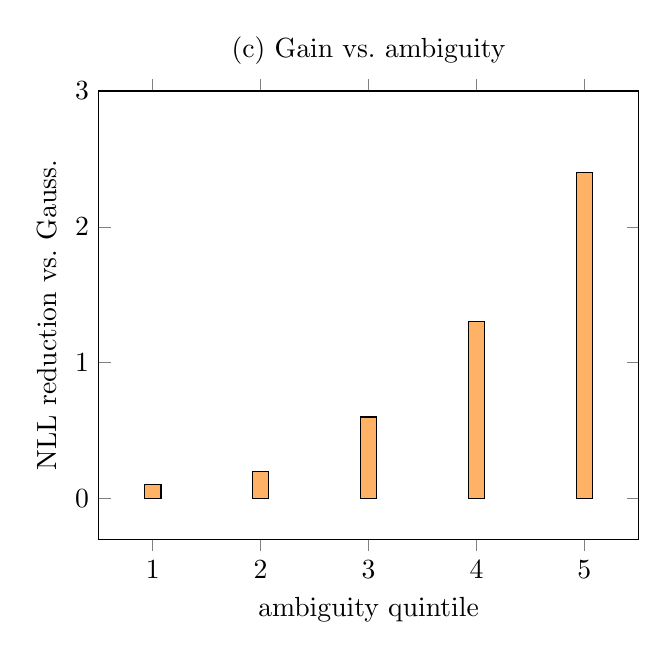
\begin{tikzpicture}
\begin{axis}[title={(c) Gain vs.\ ambiguity}, xlabel={ambiguity quintile}, ylabel={NLL reduction vs.\ Gauss.}, xmin=0.5,xmax=5.5,ymin=-0.3,ymax=3, ybar, bar width=6pt, xtick={1,...,5}]
\addplot[fill=orange!60] coordinates {(1,0.1)(2,0.2)(3,0.6)(4,1.3)(5,2.4)};
\end{axis}
\end{tikzpicture}
\caption{(a) Reliability of HPD regions (KITTI and nuScenes).
(b) ROC for flagging failed registrations using each method's confidence score (ours: sample spread; Gauss.: $\log\det\Sigma$; RANSAC: inlier ratio).
(c) Reduction in NLL relative to the Gaussian head (higher is better), binned by a per-frame ambiguity score.}
\label{fig:calib}
\end{figure}

\subsection{Ambiguous scenes}
\textbf{(i) Highway hold-out.}
We retrain on sequences 00 and 02--08 and test on 01, a highway, reporting along-track and cross-track error and NLL separately.
\emph{Expected:} \method{} samples spread along the road and stay tight across it.

\textbf{(ii) Twin places.}
We add a non-overlapping copy of each test scan, so the true posterior has two equal modes, and delete a fraction $\rho\in\{0,.25,.5\}$ of the copy's points to unbalance them.
We report mode recall and the probability mass on the original scan.
\emph{Expected:} \method{} finds both modes; the Gaussian head collapses or averages them, and RANSAC picks one.
Across all test frames, we also bin the gain over the Gaussian head by ambiguity (\cref{fig:calib}c); if multimodality is the reason, the gain should grow with ambiguity.

\subsection{Ablations}
\Cref{tab:abl} varies one design choice at a time on KITTI. We expect projective conditioning to clearly beat pose-independent features, accuracy to saturate at a few Euler steps and a few dozen samples, and the uniform rotation prior to match the yaw-only prior while making no assumption about the rotation.

\begin{table}[h]
\centering\scriptsize
\caption{Ablations on KITTI 09--10 (default in bold).}
\label{tab:abl}
\begin{tabular}{@{}llccccc@{}}
\toprule
Factor & Setting & Acc$\uparrow$ & RR$\uparrow$ & NLL$\downarrow$ & AUROC$\uparrow$ & ms/frame$\downarrow$\\
\midrule
Conditioning & pose-independent features / \textbf{projective} & \ph & \ph & \ph & \ph & \ph\\
Euler steps $K$ / samples $N$ & $K\in\{1,5,\mathbf{20},50\}$; $N\in\{8,16,\mathbf{64},256\}$ & \ph & \ph & \ph & \ph & \ph\\
Rotation prior & yaw-only / \textbf{uniform $\SO$} & \ph & \ph & \ph & \ph & \ph\\
\bottomrule
\end{tabular}
\end{table}

\subsection{Compute, data and feasibility}
\textbf{Data.} KITTI and nuScenes need about 102\,GB and 200\,GB after preprocessing.
\textbf{Software.} PyTorch, with CoFiI2P's released checkpoints and Docker image (CUDA~11.x custom operations), and \texttt{roma}.
\textbf{Hardware.} One RTX 3090 for development, and 8 NVIDIA A100s plus Digital Research Alliance of Canada clusters for training.
\textbf{Budget.} About 1 GPU-day per configuration and 10--15 GPU-days in total, plus 1--2 for retraining the backbone if needed.
\textbf{Fallback.} A 3-DoF $(x,y,\text{yaw})$ version on KITTI only, evaluated with the standard metrics (RTE, RRE, Acc, RR).

% =====================================================================
{\small
\bibliographystyle{plainnat}
\bibliography{refs}
}

\appendix
\section{AI-use disclosure}
This proposal was drafted with assistance from Claude (Anthropic), which helped with the literature search and the \LaTeX{} figures and tables.

\end{document}
